% Source: https://tex.stackexchange.com/a/684881/6880

\documentclass{standalone}
\usepackage{tikz}
\usepackage{twemojis}

\newlength{\mywidth}
\newlength{\myheight}

\newcommand{\getwh}[1]{% #1 = node name (no parens)
  \pgfextractx{\mywidth}{\pgfpointdiff{\pgfpointanchor{#1}{west}}{\pgfpointanchor{#1}{east}}}%
  \pgfextracty{\myheight}{\pgfpointdiff{\pgfpointanchor{#1}{south}}{\pgfpointanchor{#1}{north}}}%
}
  
\begin{document}
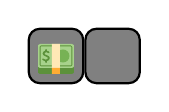
\begin{tikzpicture}
    \tikzset{nodestyle/.style={rectangle, rounded corners, draw=black, thick, fill=black!50}}
    \node[nodestyle] (node00) at (0, 0) {{\LARGE\texttwemoji{dollar banknote}}};
    \getwh{node00}% get size based on anchors
    \addtolength{\mywidth}{-0.8pt}% remove line thickness
    \addtolength{\myheight}{-0.8pt}% remove line thickness
    \node[nodestyle, right=0pt, minimum width=\mywidth, minimum height=\myheight] at (node00.east) (node01) {};
\end{tikzpicture}
\end{document}

